\hypertarget{rfidinputdialog_8h}{
\section{RFID\_\-Reader/rfidinputdialog.h File Reference}
\label{rfidinputdialog_8h}\index{RFID\_\-Reader/rfidinputdialog.h@{RFID\_\-Reader/rfidinputdialog.h}}
}
Stellt die Eingabemaske, sowie die benötigten Funktionen zum auswerten von RFID-Tags eines beliebigen Lesers zur Verfügung. 

{\tt \#include $<$QtGui$>$}\par
{\tt \#include $<$QtSql$>$}\par
{\tt \#include \char`\"{}ui\_\-rfidinputdialog.h\char`\"{}}\par
{\tt \#include \char`\"{}RFID\_\-Reader/RFID\_\-CR500.h\char`\"{}}\par


Include dependency graph for rfidinputdialog.h:\nopagebreak
\begin{figure}[H]
\begin{center}
\leavevmode
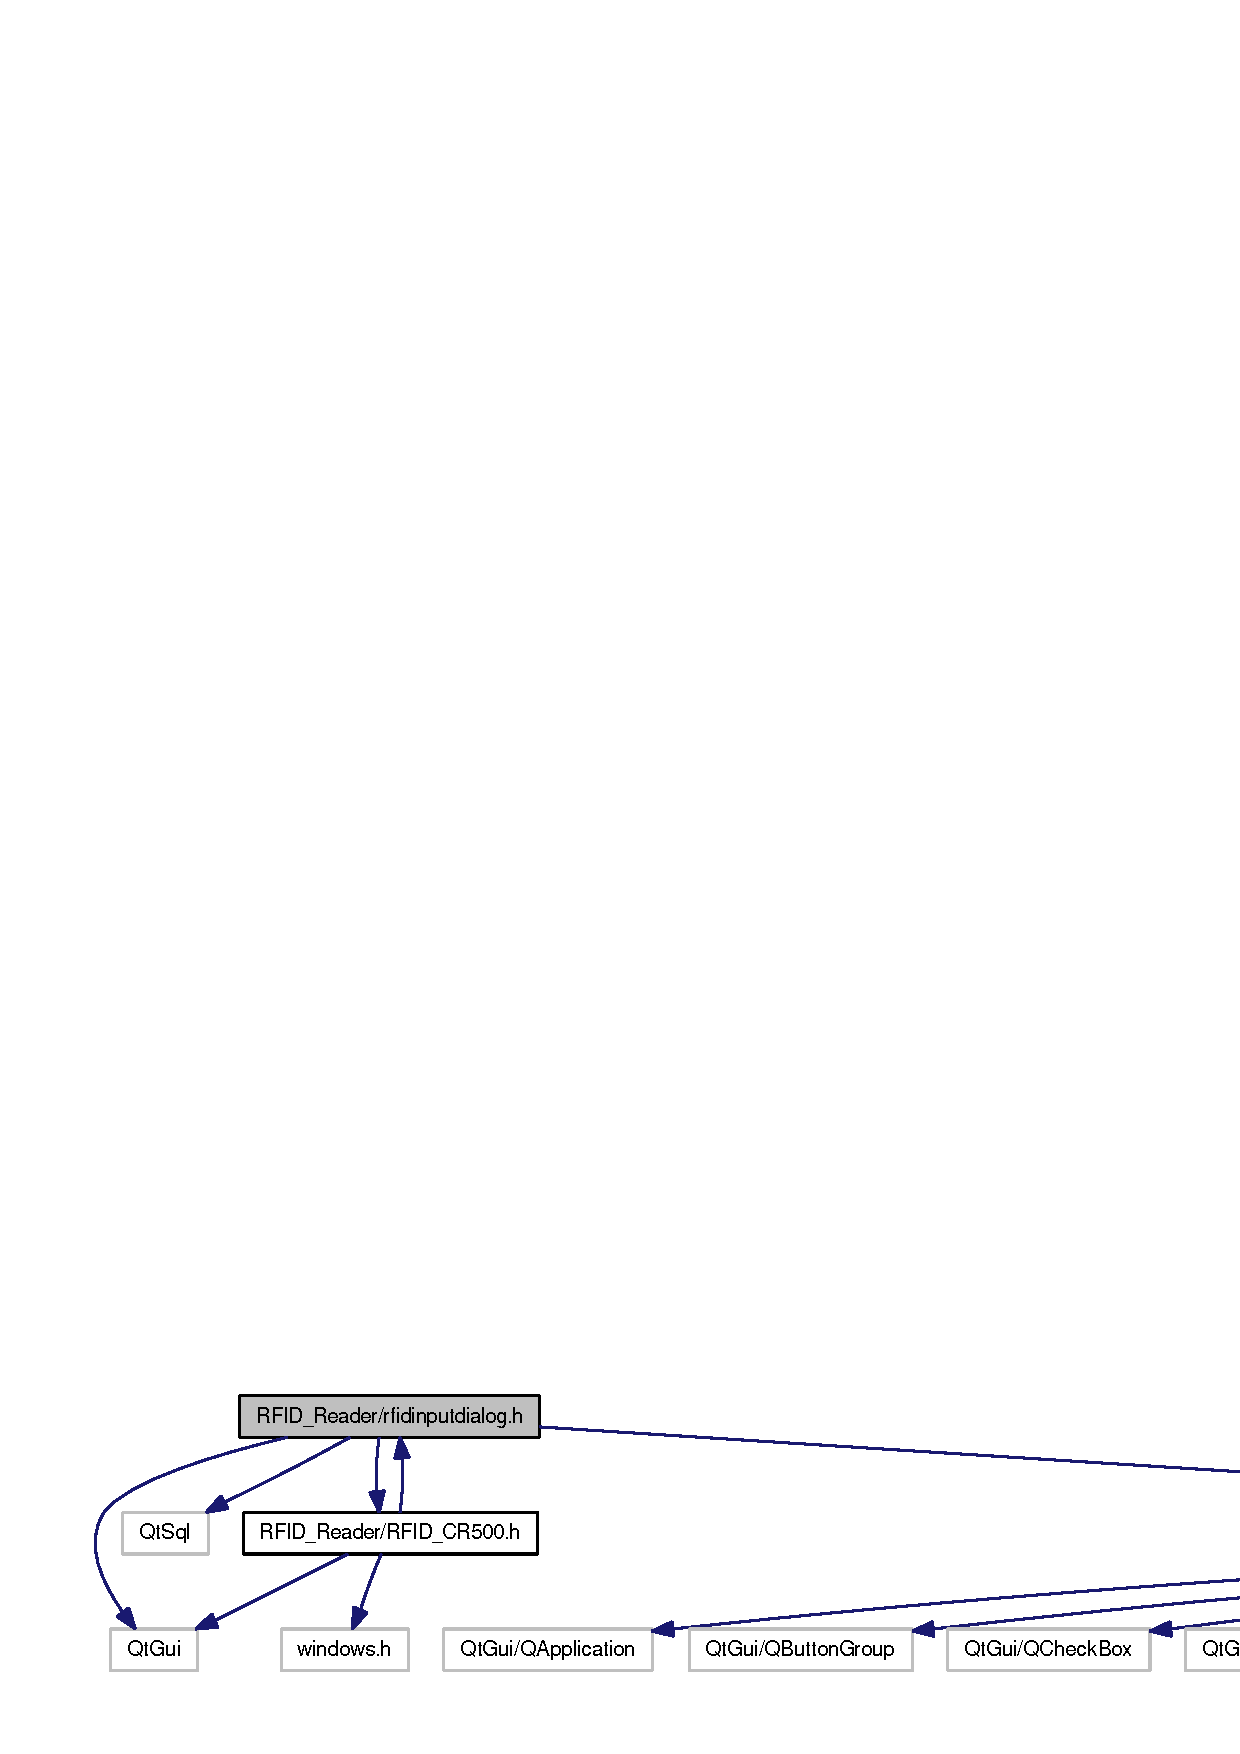
\includegraphics[width=420pt]{rfidinputdialog_8h__incl}
\end{center}
\end{figure}


This graph shows which files directly or indirectly include this file:\nopagebreak
\begin{figure}[H]
\begin{center}
\leavevmode
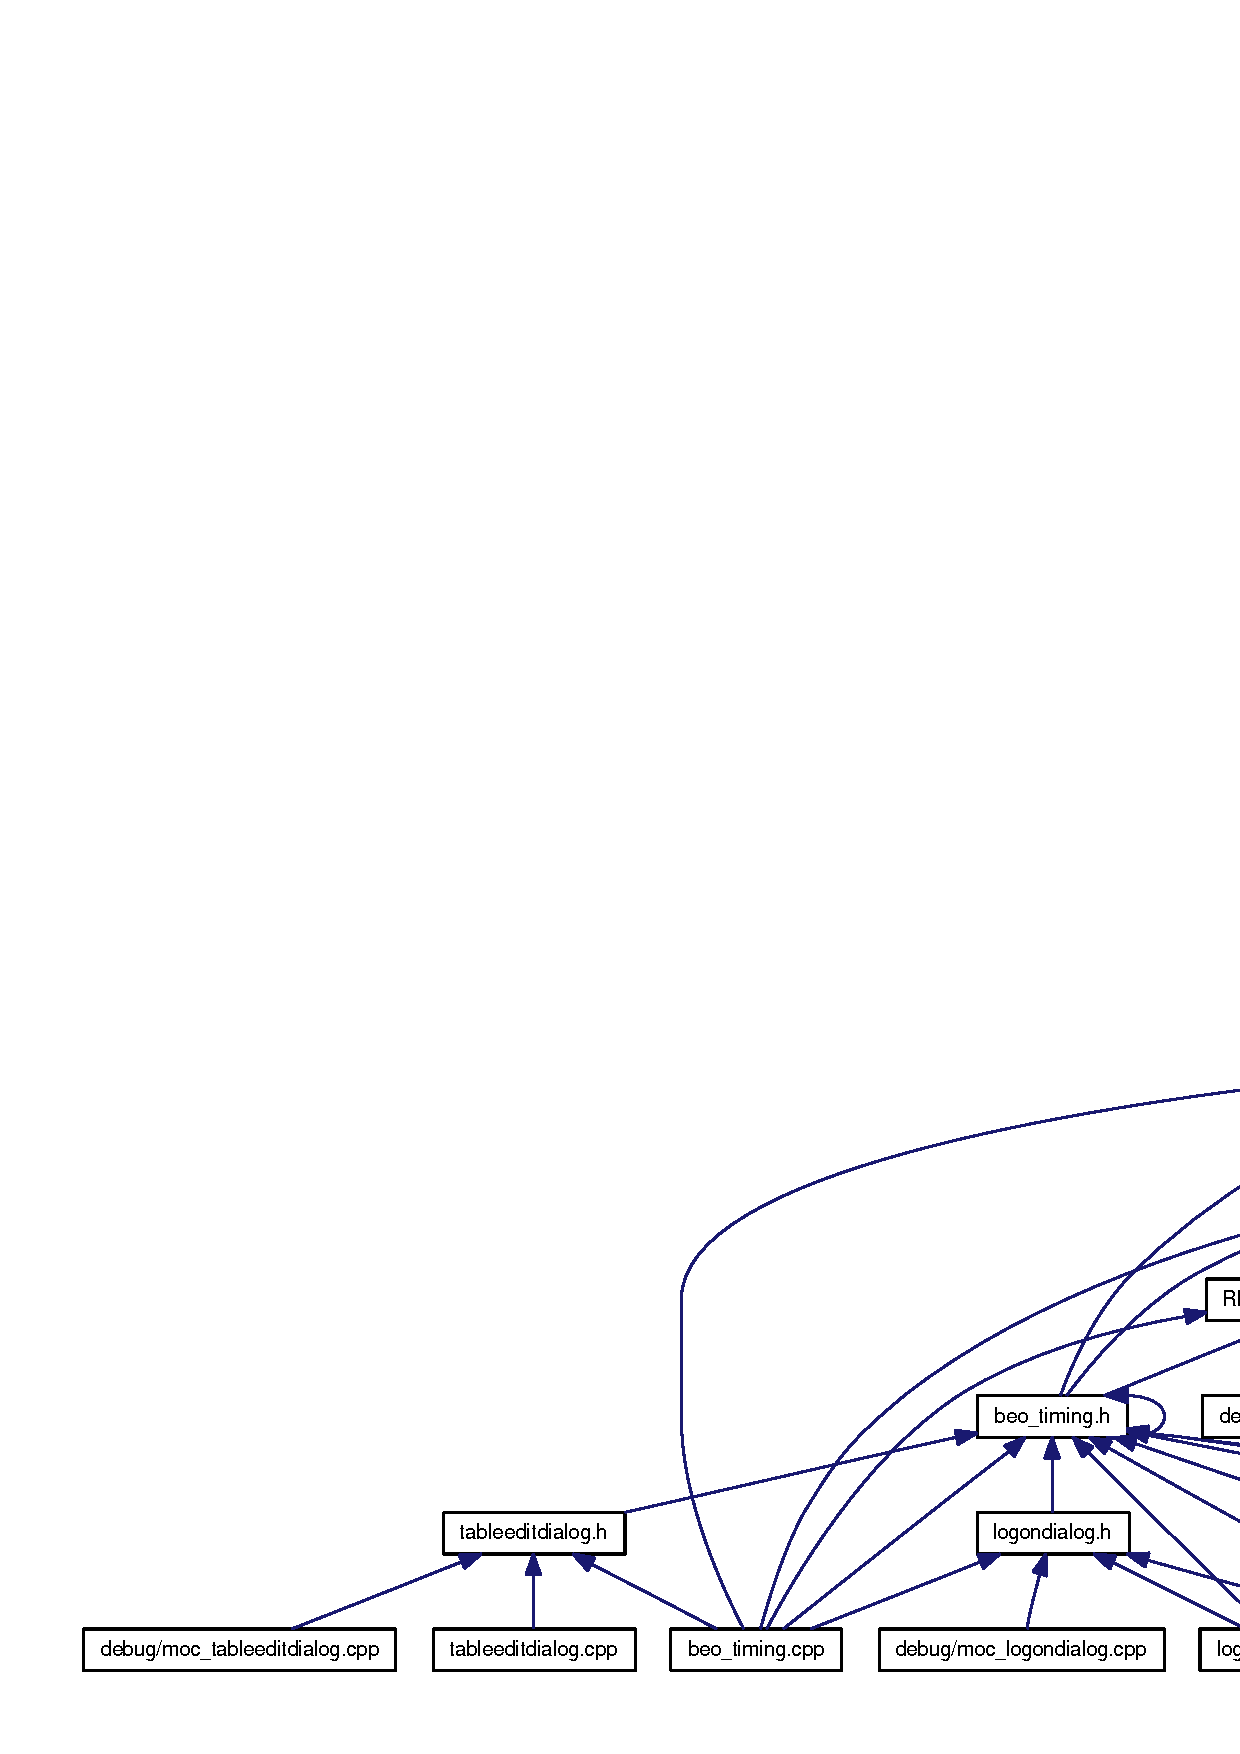
\includegraphics[width=420pt]{rfidinputdialog_8h__dep__incl}
\end{center}
\end{figure}
\subsection*{Classes}
\begin{CompactItemize}
\item 
class \hyperlink{class_r_f_i_d_input_dialog}{RFIDInputDialog}
\begin{CompactList}\small\item\em Stellt die Eingabemaske, sowie die benötigten Funktionen zum auswerten von RFID-Tags eines beliebigen Lesers zur Verfügung. \item\end{CompactList}\end{CompactItemize}


\subsection{Detailed Description}
Stellt die Eingabemaske, sowie die benötigten Funktionen zum auswerten von RFID-Tags eines beliebigen Lesers zur Verfügung. 

\begin{Desc}
\item[Version:]1.0 \end{Desc}
\begin{Desc}
\item[Date:]09.06.2008 \end{Desc}
\begin{Desc}
\item[Author:]R.Zoss\end{Desc}
Copyright (C) 2008 Rico Zoss

This file is part of BEO-Timing Managementsoftware.

BEO-Timing Managementsoftware is free software: you can redistribute it and/or modify it under the terms of the GNU General Public License as published by the Free Software Foundation, either version 3 of the License, or (at your option) any later version.

BEO-Timing Managementsoftware is distributed in the hope that it will be useful, but WITHOUT ANY WARRANTY; without even the implied warranty of MERCHANTABILITY or FITNESS FOR A PARTICULAR PURPOSE. See the GNU General Public License for more details.

You should have received a copy of the GNU General Public License along with BEO-Timing Managementsoftware. If not, see $<$\href{http://www.gnu.org/licenses/}{\tt http://www.gnu.org/licenses/}$>$. 

Definition in file \hyperlink{rfidinputdialog_8h-source}{rfidinputdialog.h}.